\section{Összefoglalás}

A szoftver tehát a bejelentőben felsorolt funkciókat megvalósítja, jelenlegi
állapotában alkalmas egy drónflotta térkép segítségével történő vizuális
kezelésére, a drónokon lévő műszerek méréseinek megjelenítésére.

Többször is volt tesztelve valódi drónokkal, ezek közül egyik alkalomra a
2017-ben Budapesten megrendezésre kerülő FINA Vizes Világbajnokság megnyitójának
főpróbáján került sor. A mellékelt képek mutatják a drónok elhelyezkedését a
rakparton (\ref{fig:fina_launch}. ábra), és az ezzel a képpel közel egy időben készült
képernyőfelvételt a szoftver akkor aktuális állapotáról
(\ref{fig:fina_launch_screen}. ábra), melyen megjelennek az elérhető kopterek.

\begin{figure}[H]
  \center
  \includegraphics[width=\textwidth]{fina_launch.jpg}
  \caption{Egy Duna-parti felszállás előtt}
  \label{fig:fina_launch}
\end{figure}

\begin{figure}[H]
  \center
  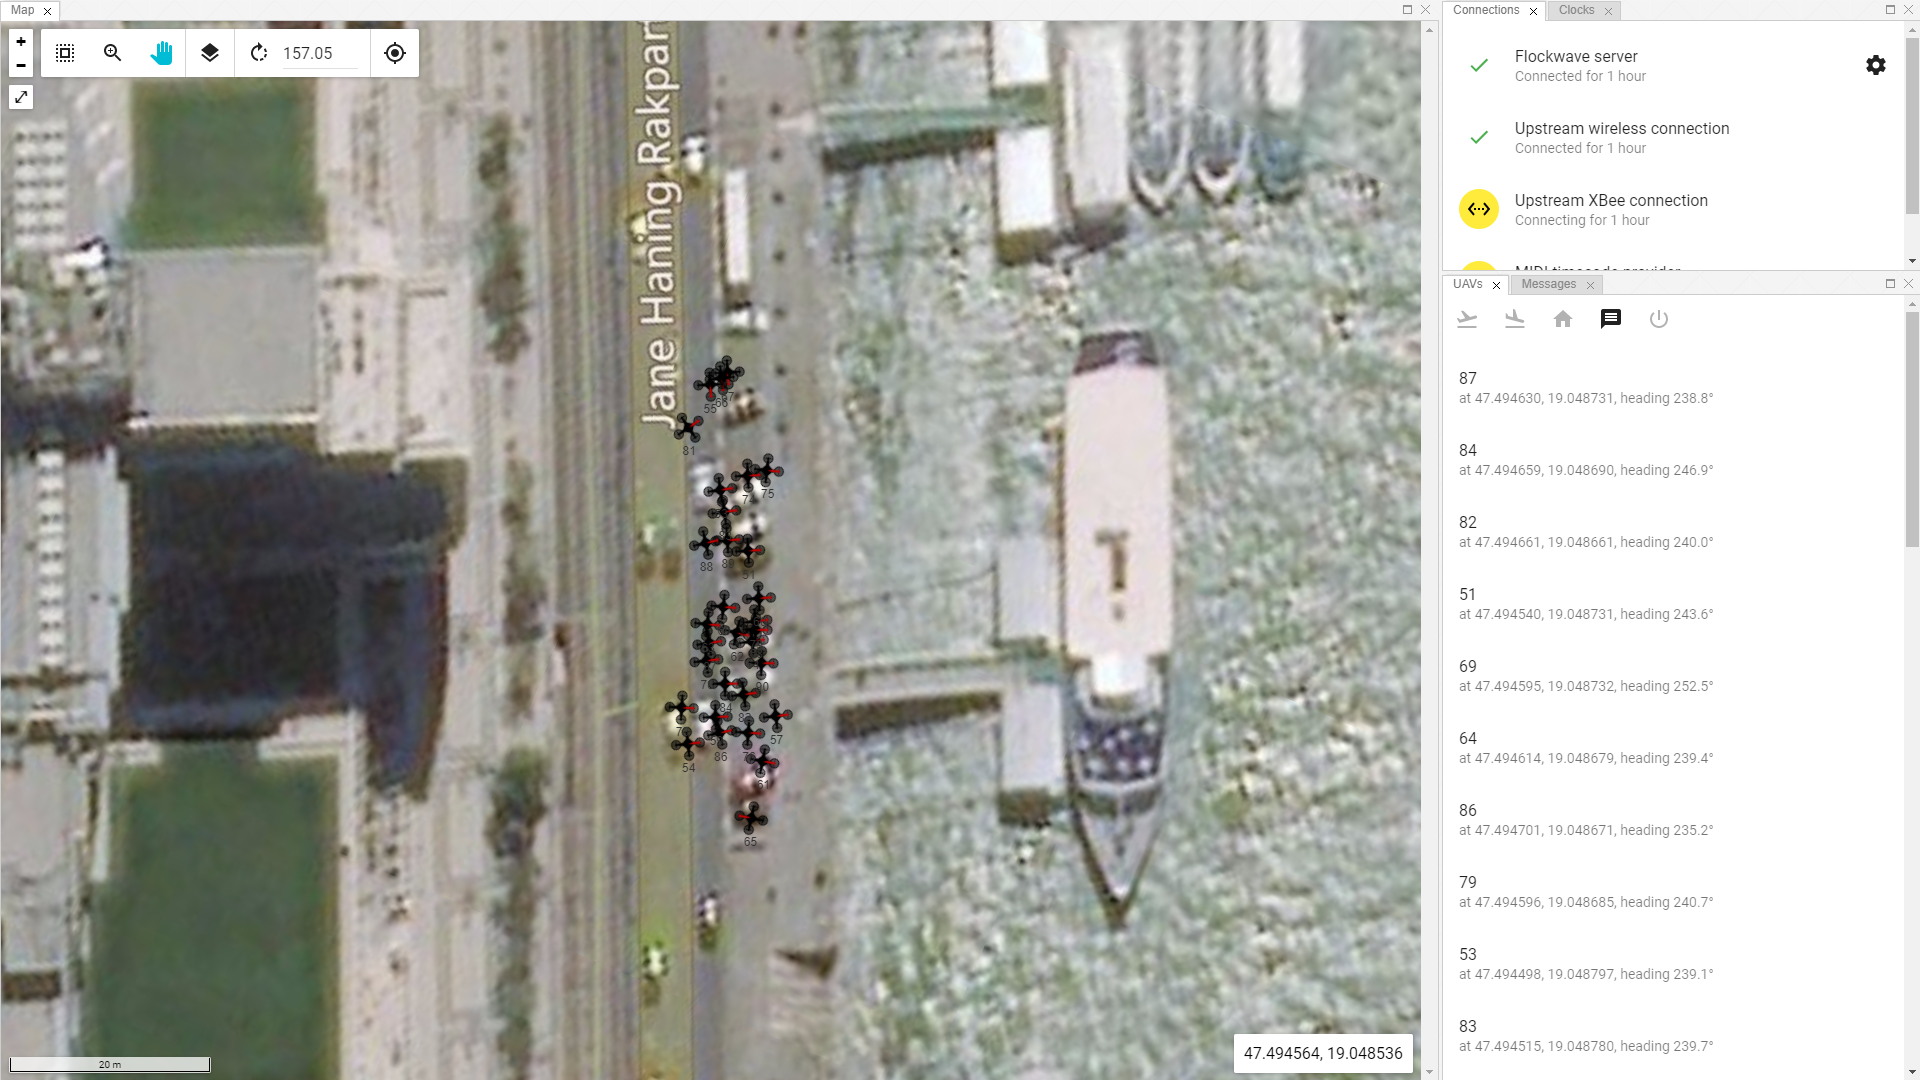
\includegraphics[width=\textwidth]{fina_launch_screen.png}
  \caption{Egy Duna-parti felszállás előtt (képernyőkép)}
  \label{fig:fina_launch_screen}
\end{figure}

A szoftver fejlesztése továbbra is folyamatosan zajlik, állandóan új és új
funkciókkal bővül és időről időre tesztelésre is kerül.
